\newslide{Schematics -- Antenna and PreAmplifier}{
	\begin{block}{}
		%\centering
		\begin{tikzpicture}
			\node [] (complete) {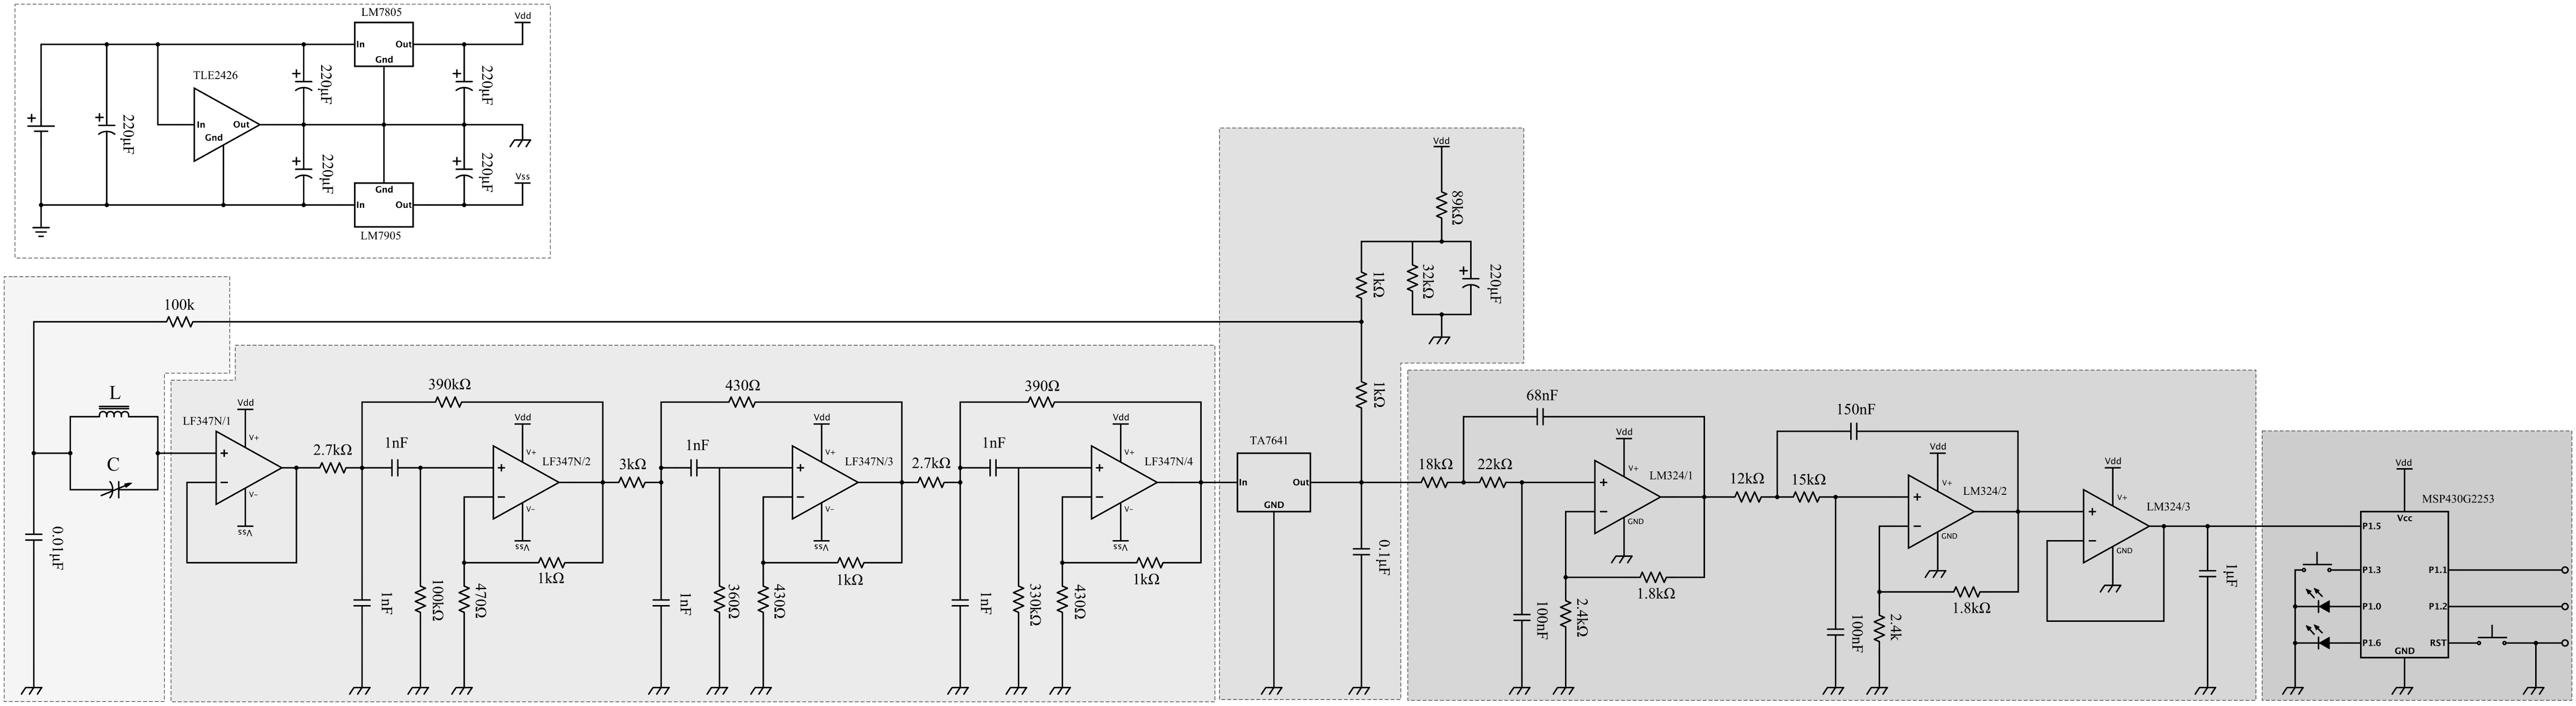
\includegraphics[width=12cm]{img/receiver.png}};
			\node [rectangle,draw, dashed, minimum width=5.7cm, minimum height=2.15cm, xshift=-3.17cm, yshift=-0.64cm] (lookat) {};
			\node [rectangle,draw, dashed, at=(complete.south west), anchor=north west, yshift=-1cm] (part1) {
\includegraphics[width=12.5cm]{img/receiver_1.png}};
			\draw [dashed](lookat.south west) -- (part1.north west);
			\draw [dashed](lookat.south east) -- (part1.north east);
			\node [at=(part1.east), anchor=west] (graph) {
			\begin{tikzpicture}

				\begin{semilogxaxis}[xlabel={\scriptsize Frequency (Hz)}, ylabel={\scriptsize Magnitude (dB)},
				                     xmin=10^3, xmax=10^8, ymin=-150, ymax=60, tick label style={font=\scriptsize},
				                     height=6cm, width=6cm, grid=both,, grid style={color=gray!50, dotted},
				                     xminorticks=true, scaled ticks=true,log basis x=10,enlargelimits=false,title={PreAmplifier Characteristic}]
					\addplot[mark=none,line width=1.5] file {../ch2/img/filter1.txt};
				\end{semilogxaxis}
			
			\end{tikzpicture}
			};
		\end{tikzpicture}
	\end{block}
}
